\chapter{Appendix}

\begin{figure}[htbp]
    \centering
    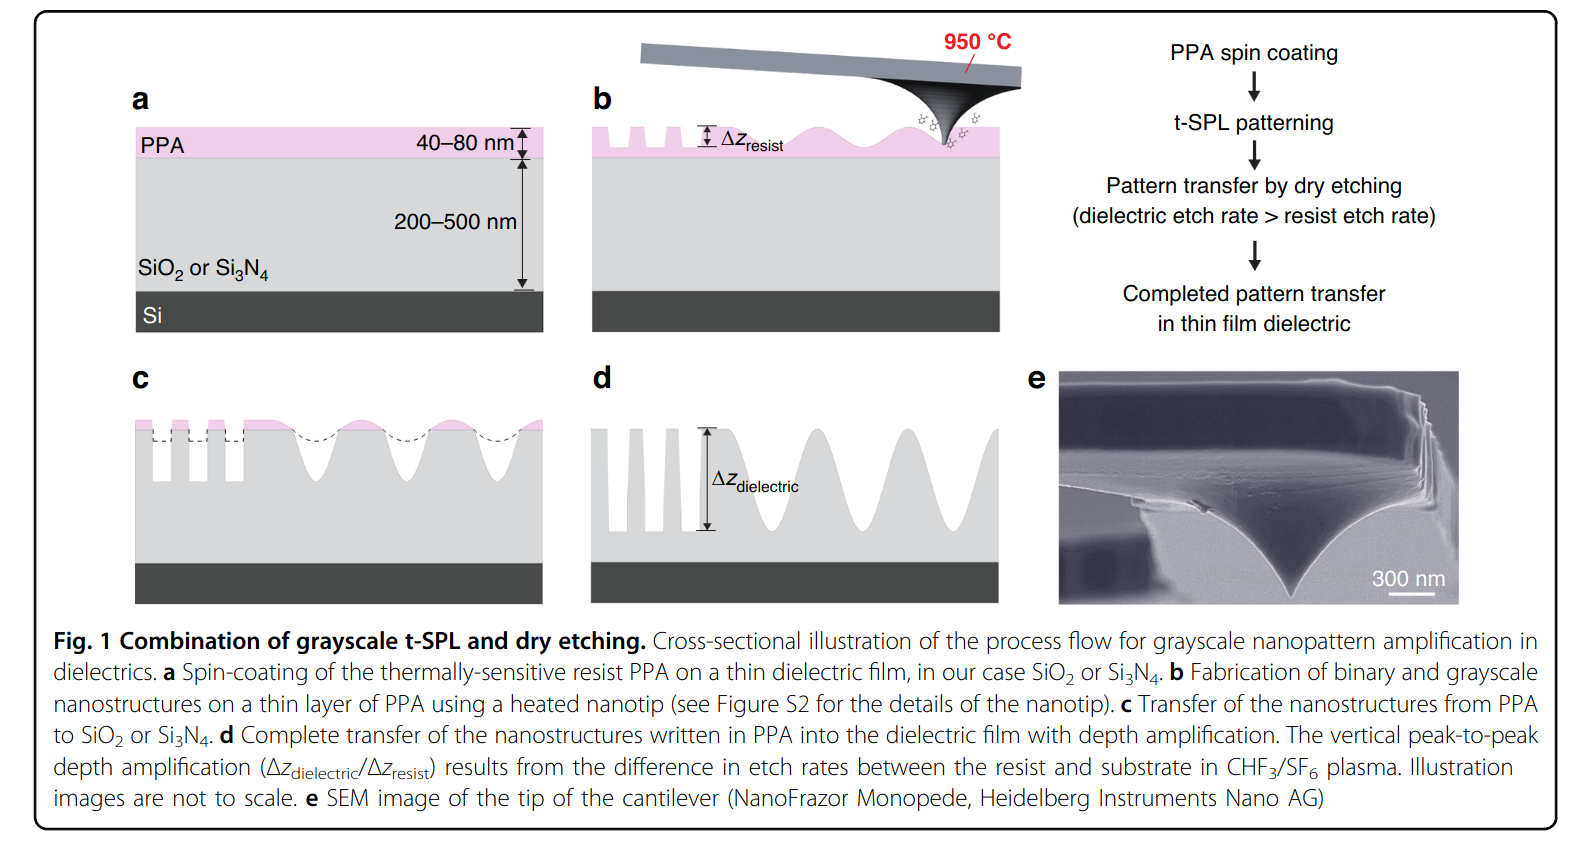
\includegraphics[width=\textwidth]{figures/Erbas2024.png}
    \caption{Grayscale nanopattern amplification \cite{Erbas2024}.}
    \label{fig:erbas2024}
\end{figure}

\begin{figure}[htbp]
    \centering
    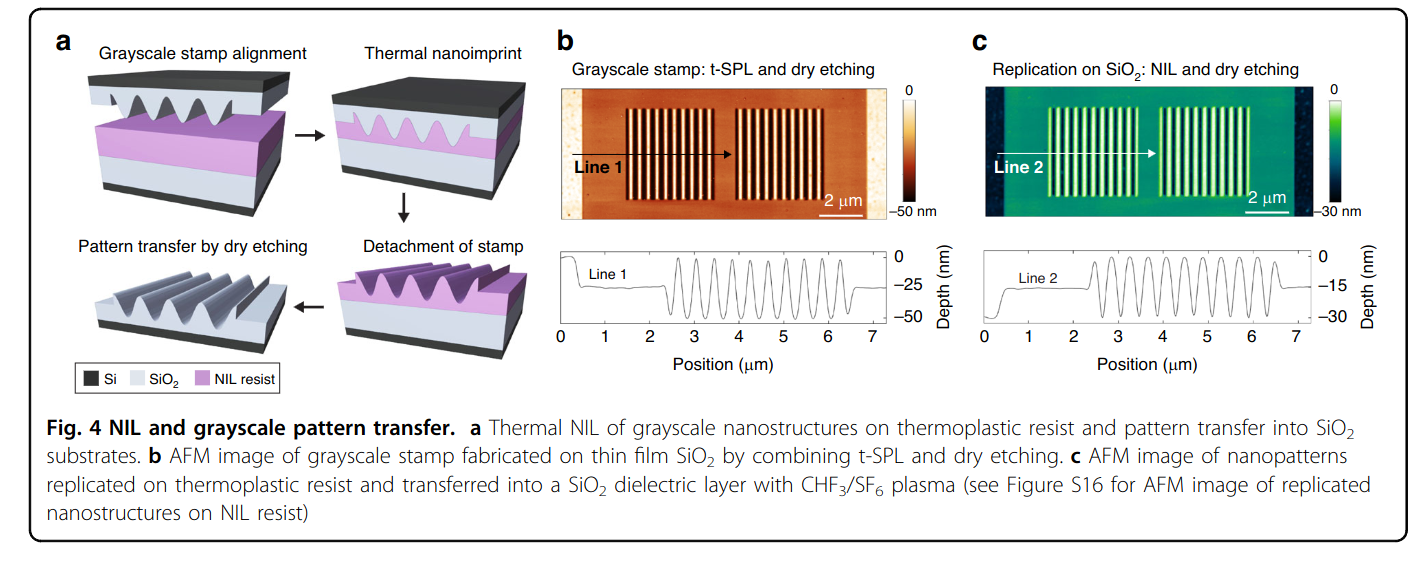
\includegraphics[width=\textwidth]{figures/Erbas2024_2.png}
    \caption{An example of a 3D nanopattern following the formulation of eq \ref{eq:grating}. \cite{Erbas2024}.}
    \label{fig:erbas2024_2}
\end{figure}

\begin{figure}[htbp]
    \centering
    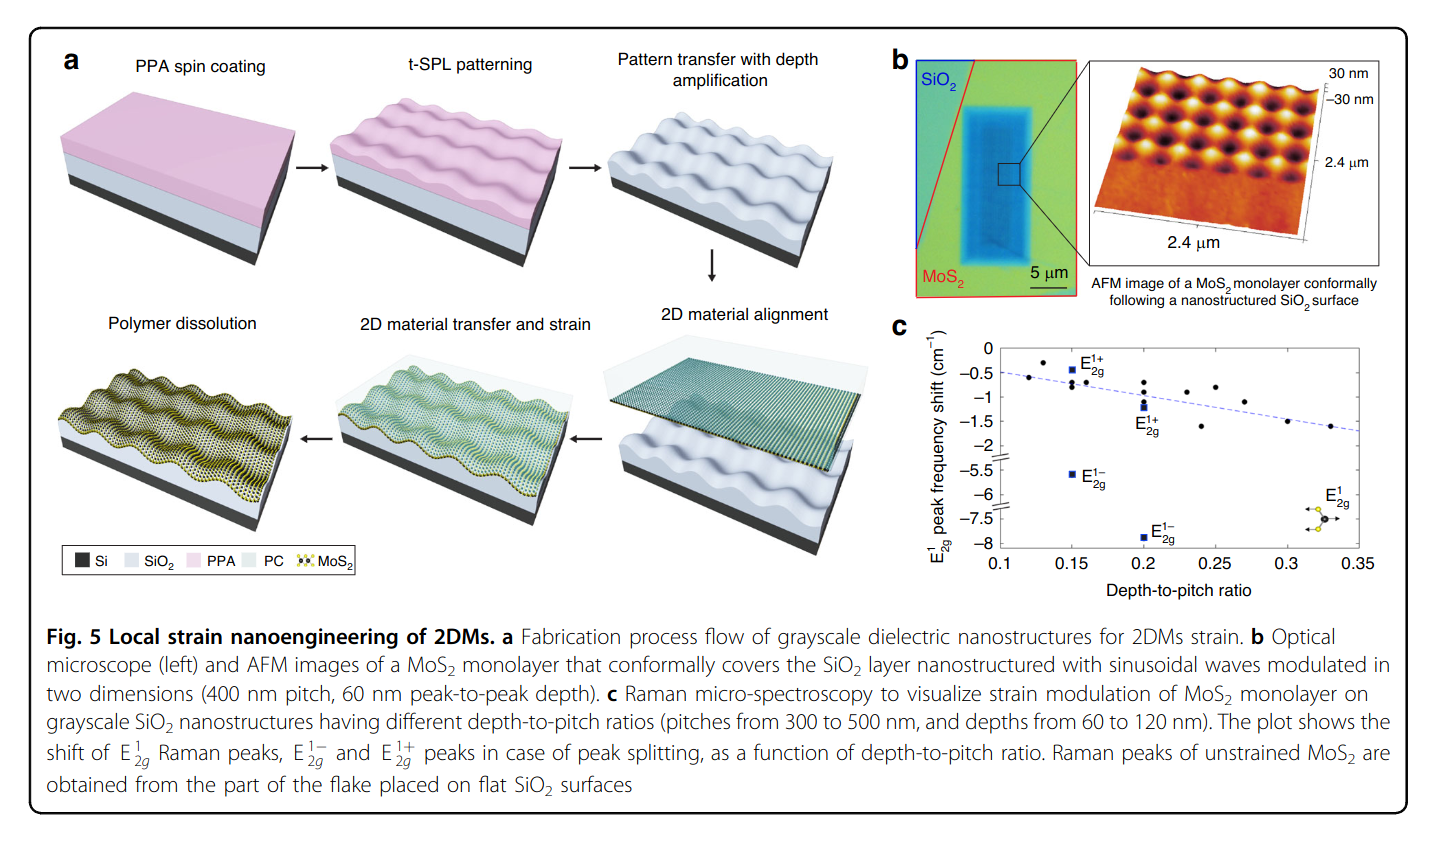
\includegraphics[width=\textwidth]{figures/Erbas2024_3.png}
    \caption{An example of a grayscale nanoimprint-lithography of grayscale mask. \cite{Erbas2024}.}
    \label{fig:erbas2024_3}
\end{figure}

\section{Additional Convergence Tests}

This section provides additional convergence tests for the RCWA implementation. Figures \ref{fig:conv_1000_1} through \ref{fig:conv_1000_3} display the convergence sweeps for a grating of height 1000 nm. Figures \ref{fig:conv_nosub_1} through \ref{fig:conv_nosub_6} show the convergence tests performed without subpixel smoothing.

\subsection{Convergence Tests for 1000 nm Grating}

\begin{figure}[htbp]
    \centering
    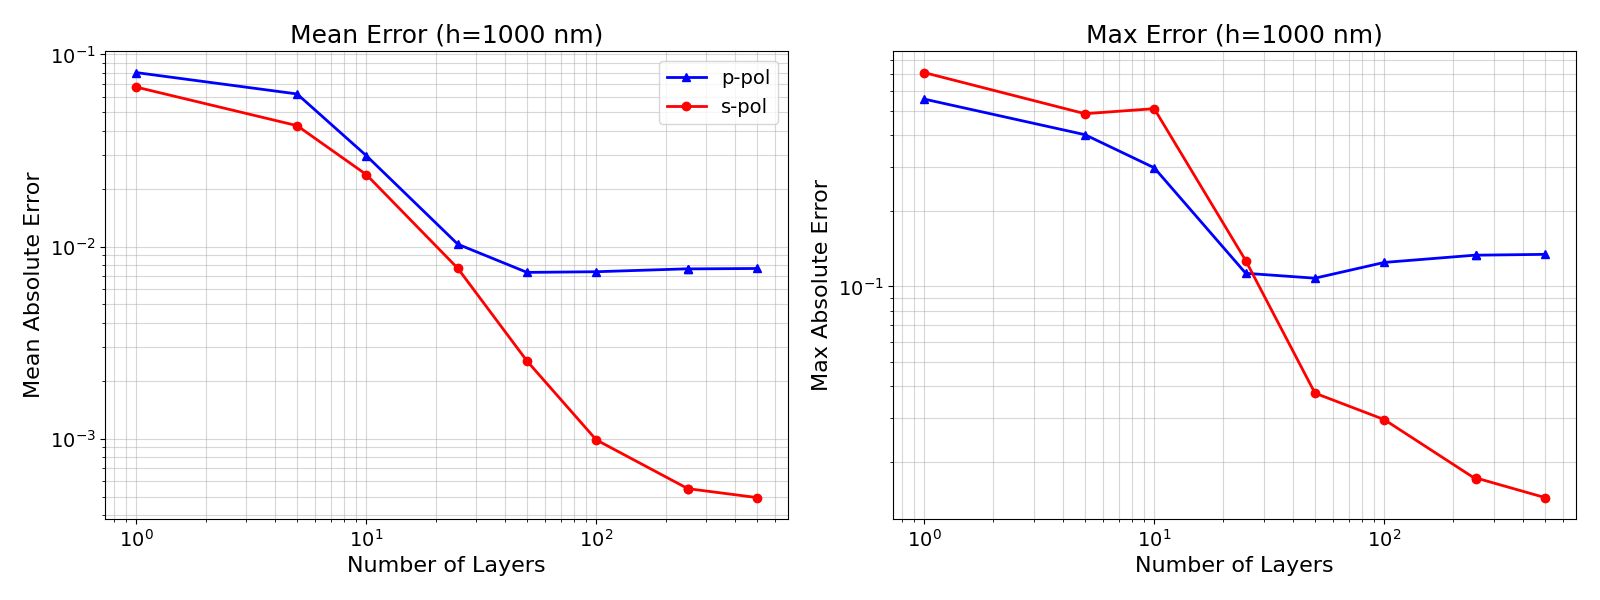
\includegraphics[width=0.85\textwidth]{figures/convergence/convergence_num_layers_1000nm.png}
    \caption{Convergence as a function of the number of staircase layers for a grating of height 1000 nm.}
    \label{fig:conv_1000_1}
\end{figure}

\begin{figure}[htbp]
    \centering
    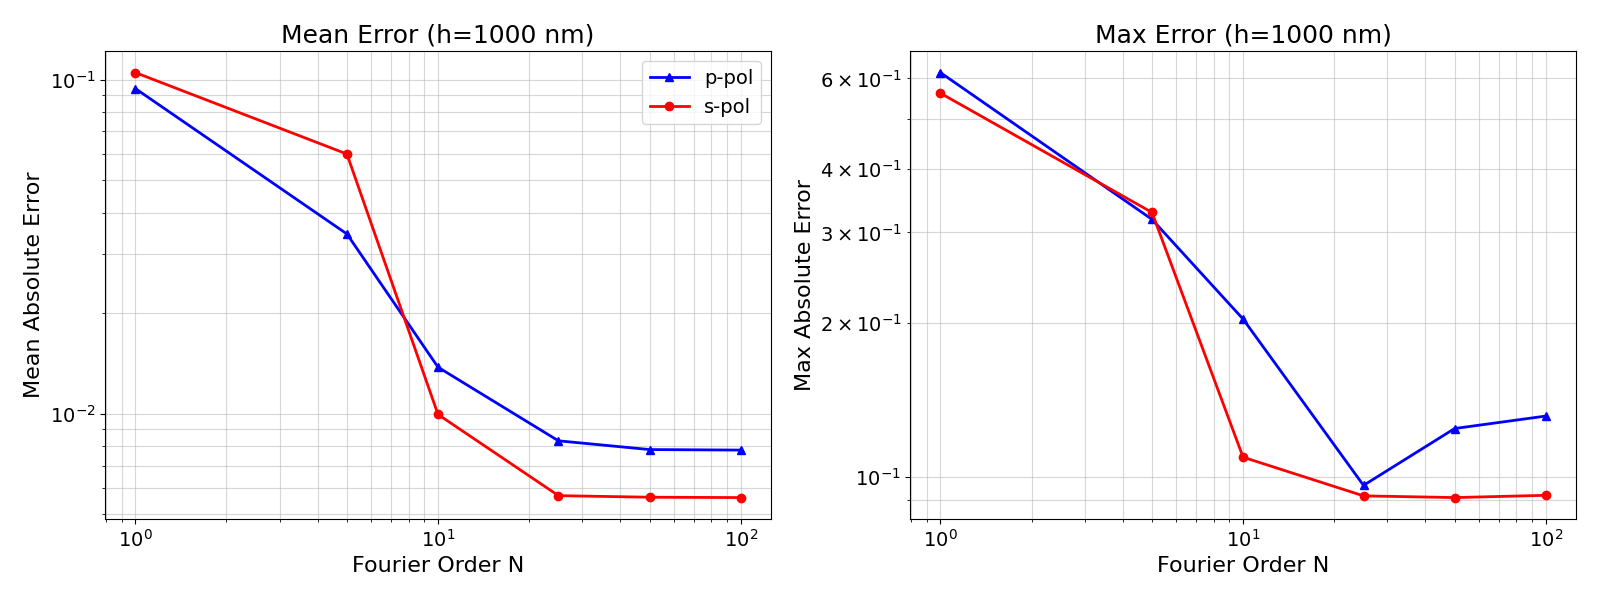
\includegraphics[width=0.85\textwidth]{figures/convergence/convergence_order_N_1000nm.png}
    \caption{Convergence as a function of the number of Fourier orders for a grating of height 1000 nm.}
    \label{fig:conv_1000_2}
\end{figure}

\begin{figure}[htbp]
    \centering
    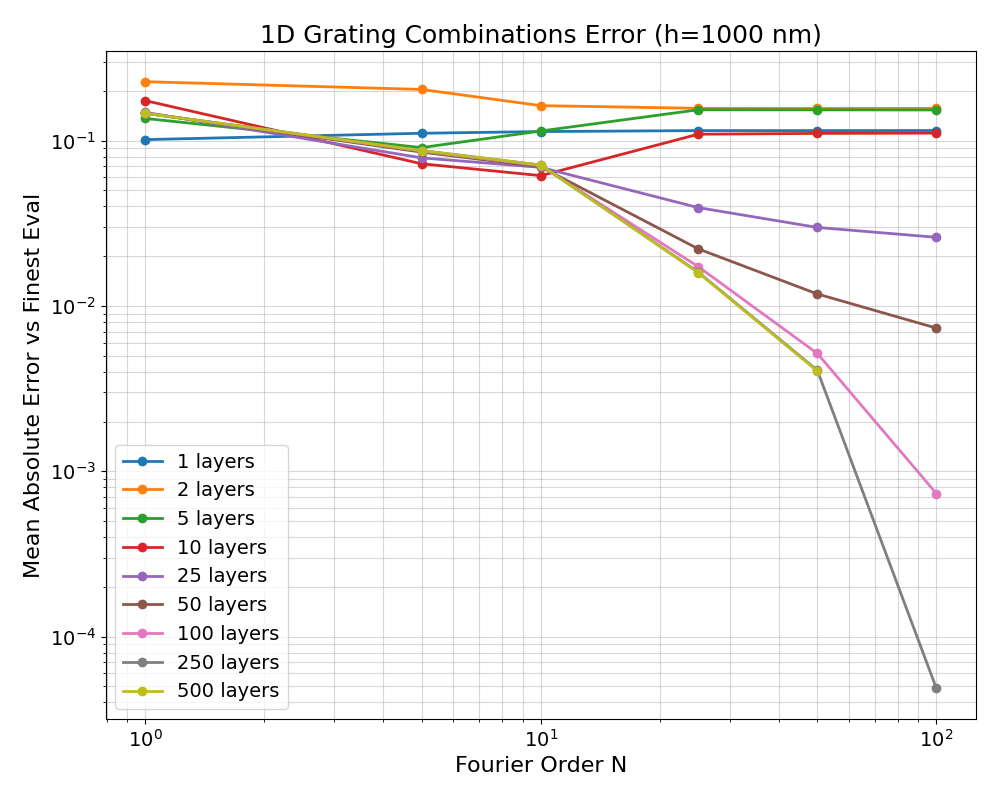
\includegraphics[width=0.48\textwidth]{figures/convergence/sweep_combination_1000nm.png}
    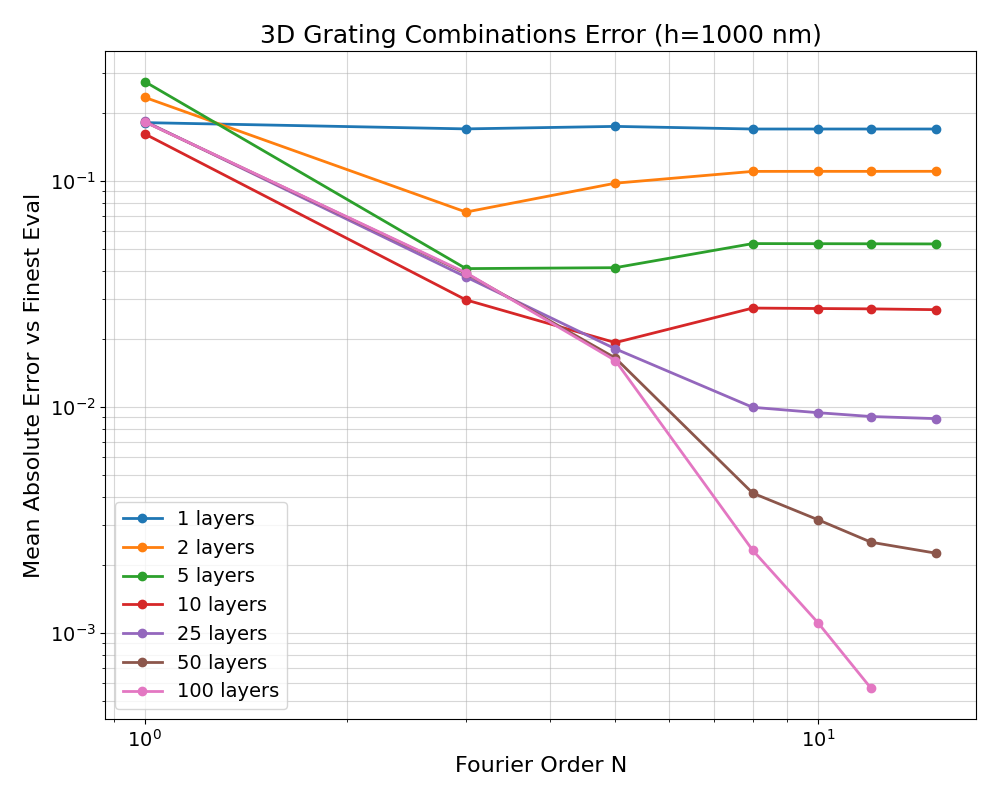
\includegraphics[width=0.48\textwidth]{figures/convergence/sweep_combination_3d_1000nm.png}
    \caption{Convergence sweeps and combinations for the 1000 nm grating structure. Left: 1D sweep combinations. Right: 3D convergence combinations.}
    \label{fig:conv_1000_3}
\end{figure}

\clearpage

\subsection{Convergence Tests without Subpixel Smoothing}

\begin{figure}[htbp]
    \centering
    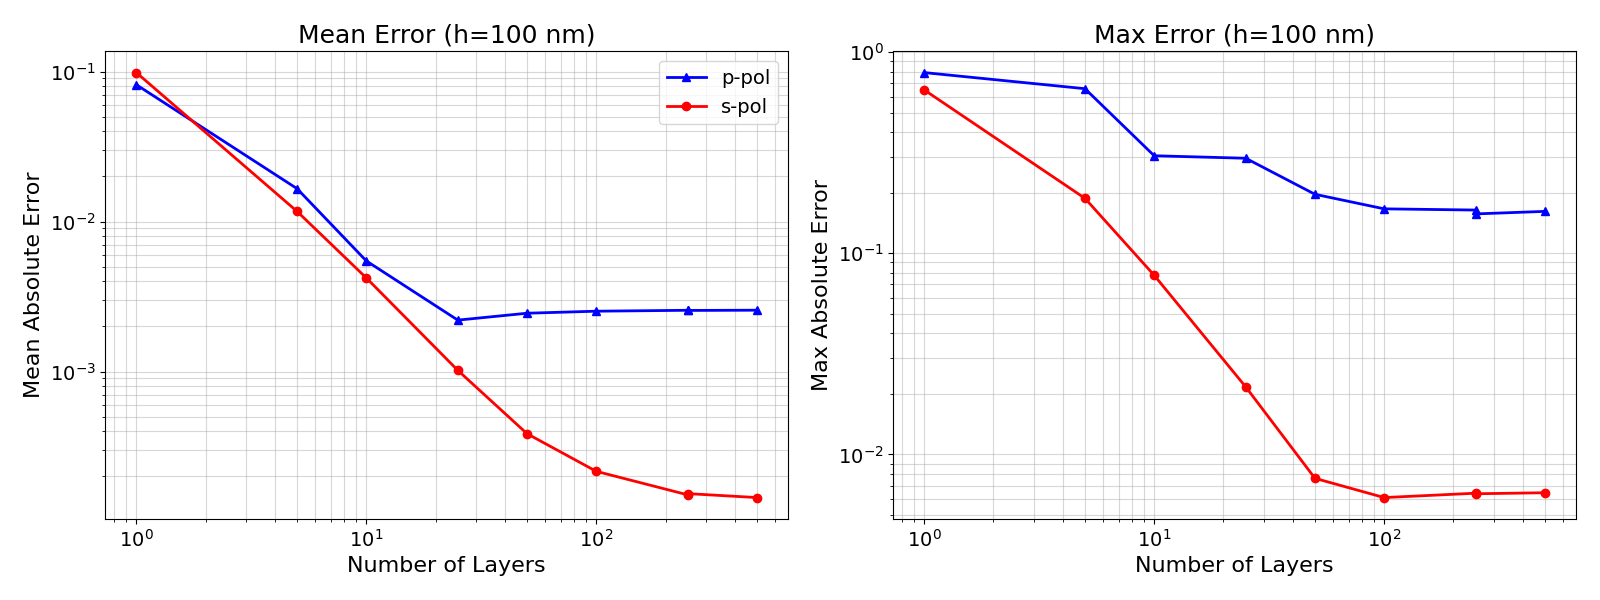
\includegraphics[width=0.85\textwidth]{figures/convergence/convergence_num_layers_no_subpixel_100nm.png}
    \caption{Convergence as a function of the number of staircase layers for a 100 nm grating without subpixel smoothing.}
    \label{fig:conv_nosub_1}
\end{figure}

\begin{figure}[htbp]
    \centering
    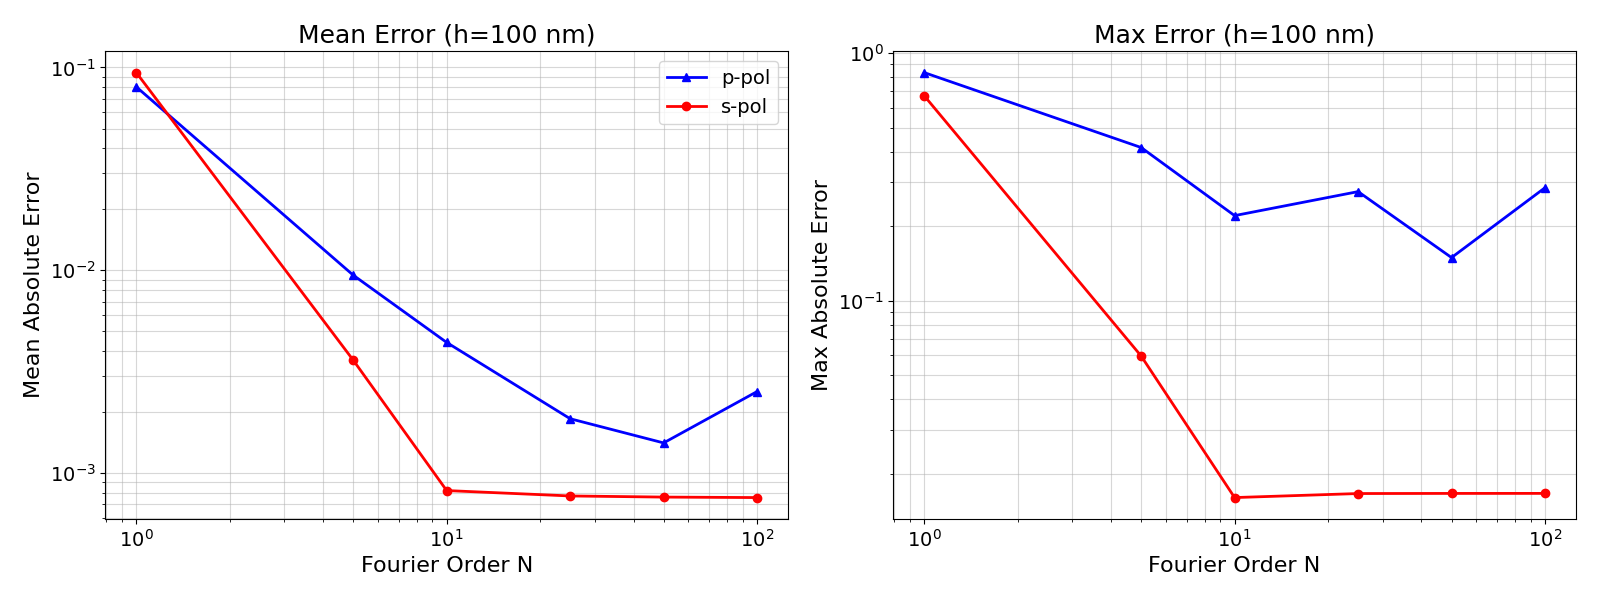
\includegraphics[width=0.85\textwidth]{figures/convergence/convergence_order_N_no_subpixel_100nm.png}
    \caption{Convergence as a function of the number of Fourier orders for a 100 nm grating without subpixel smoothing.}
    \label{fig:conv_nosub_2}
\end{figure}

\begin{figure}[htbp]
    \centering
    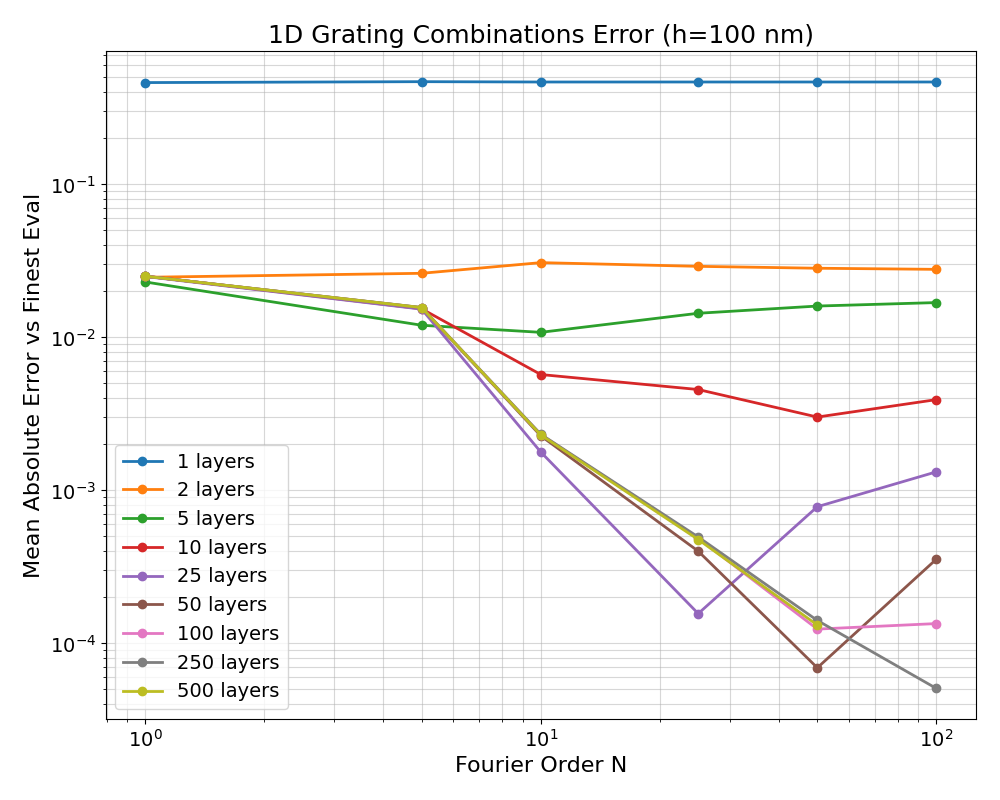
\includegraphics[width=0.48\textwidth]{figures/convergence/sweep_combination_no_subpixel_100nm.png}
    \caption{1D sweep combinations for the 100 nm grating without subpixel smoothing.}
    \label{fig:conv_nosub_3}
\end{figure}

\begin{figure}[htbp]
    \centering
    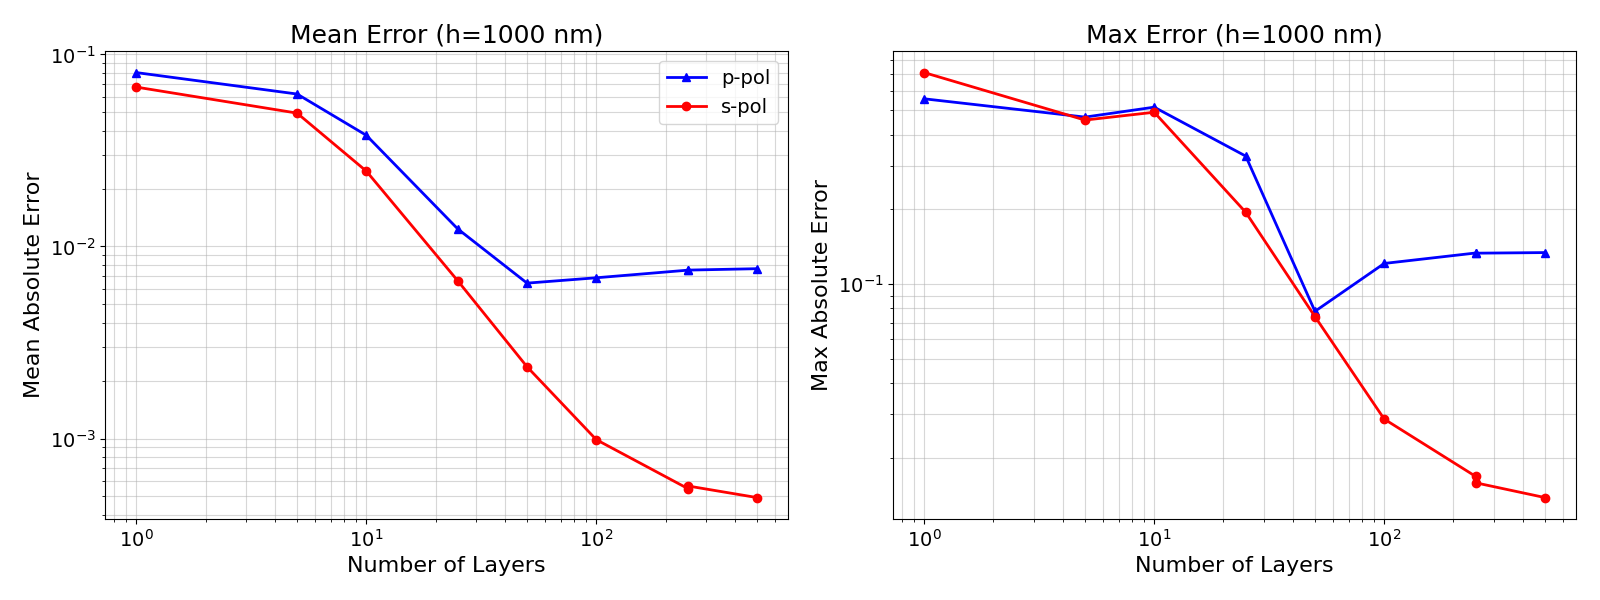
\includegraphics[width=0.85\textwidth]{figures/convergence/convergence_num_layers_no_subpixel_1000nm.png}
    \caption{Convergence as a function of the number of staircase layers for a 1000 nm grating without subpixel smoothing.}
    \label{fig:conv_nosub_4}
\end{figure}

\begin{figure}[htbp]
    \centering
    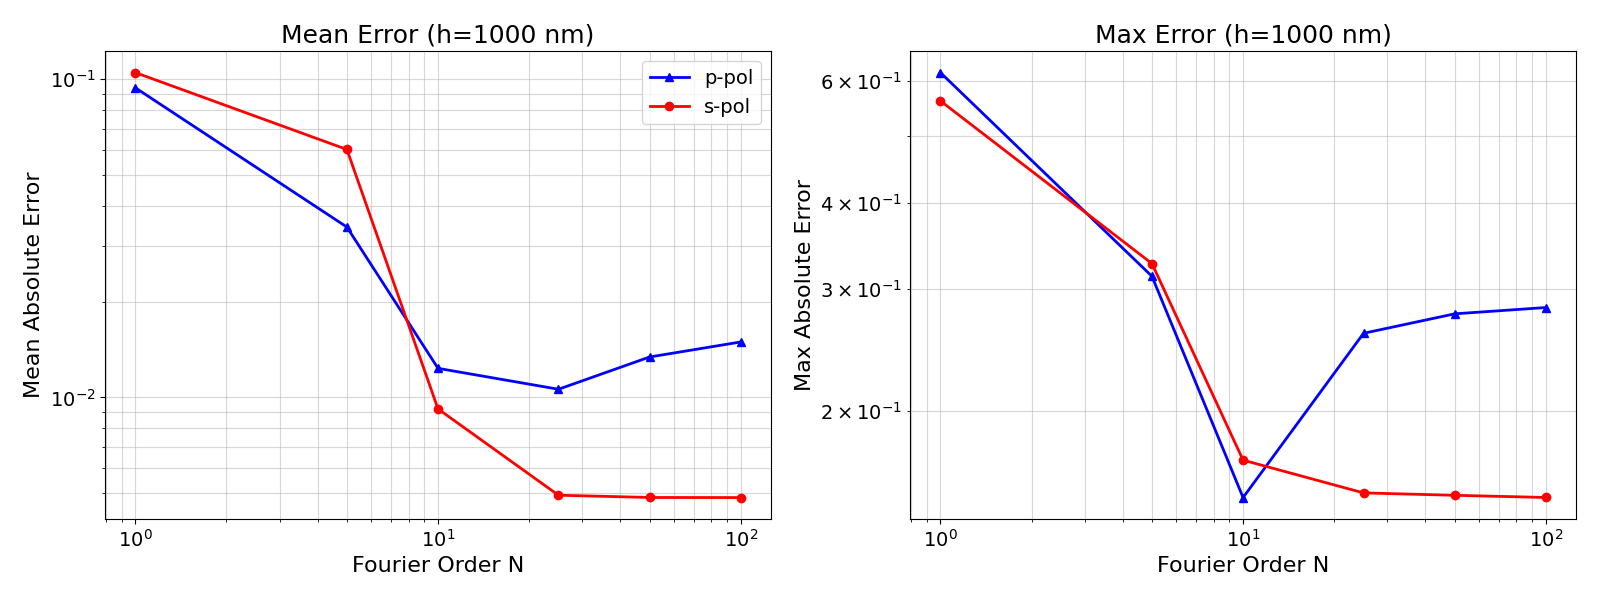
\includegraphics[width=0.85\textwidth]{figures/convergence/convergence_order_N_no_subpixel_1000nm.png}
    \caption{Convergence as a function of the number of Fourier orders for a 1000 nm grating without subpixel smoothing.}
    \label{fig:conv_nosub_5}
\end{figure}

\begin{figure}[htbp]
    \centering
    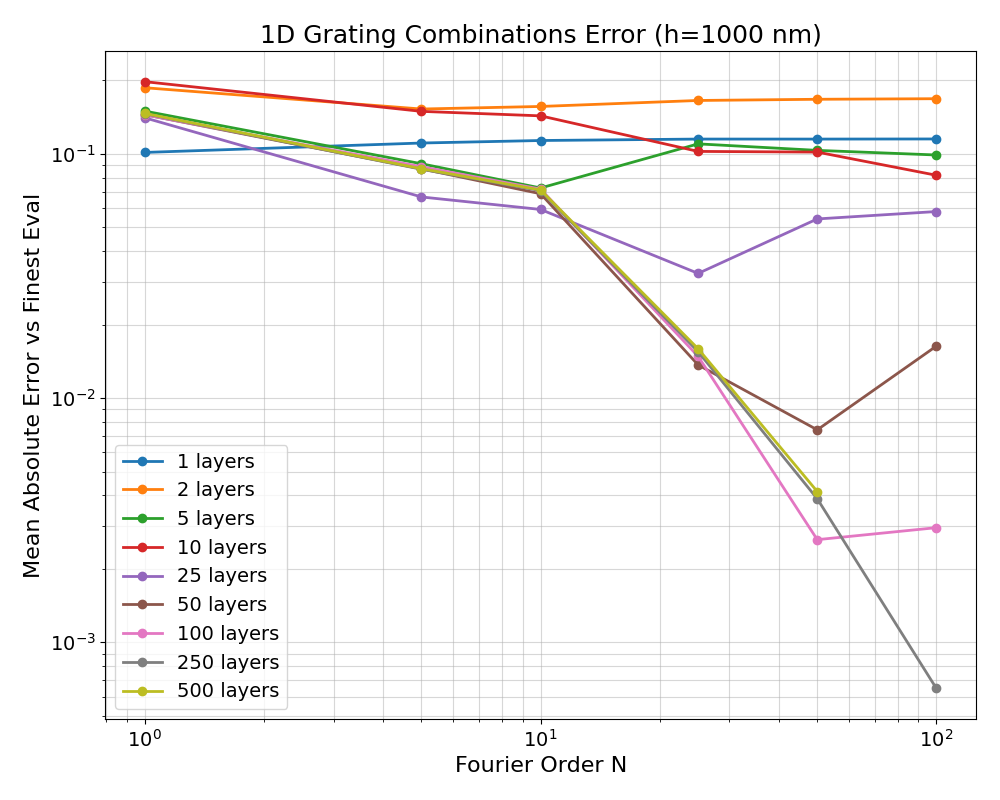
\includegraphics[width=0.48\textwidth]{figures/convergence/sweep_combination_no_subpixel_1000nm.png}
    \caption{1D sweep combinations for the 1000 nm grating without subpixel smoothing.}
    \label{fig:conv_nosub_6}
\end{figure}
\clearpage


